\documentclass[final]{beamer}

\usepackage{graphicx}
\usepackage{fancybox}
\graphicspath{{./figures/}}
\usepackage{caption}
\usepackage{subcaption}
\usepackage{amsmath}
\usepackage{bbm}
\usepackage{units}
\usepackage{tikz}
\usetikzlibrary{shapes,arrows}

\usetheme{NST}
\captionsetup{font=small,labelfont=small, labelfont={color=prime,sf}}

\usefonttheme{professionalfonts} % using non standard fonts for beamer
\usepackage[orientation=landscape,size=custom,width=121.92,height=91.44,scale=1.3]{beamerposter}
% Display a grid to help align images
%\beamertemplategridbackground[1 in]

\usepackage{lipsum}
\usepackage[absolute,overlay]{textpos}
\setlength{\TPHorizModule}{1 in}
\setlength{\TPVertModule}{1 in}

\title{Roll and height control for legged locomotion on the water surface}
\author{$\mathsf{^1}$Nitish Thatte \and $\mathsf{^1}$Mahdi Khoramshahi \and $\mathsf{^2}$Auke Isjpeert \and  $\mathsf{^1}$Metin Sitti}
\institute{$\mathsf{^1}$Carnegie Mellon University \hspace{1EM} $\mathsf{^2}$\'{E}cole Polytechnique F\'{e}d\'{e}rale de Lausanne
}

\footer{\texttt{nitisht@andrew.cmu.edu, m80.khoramshahi@gmail.com,auke.ijspeert@epfl.ch, metin@cmu.edu}}

\begin{document}

\begin{textblock}{12}(32.5,1.25)
    \includegraphics[height = 1.75in]{Nanorobotics_lab_logo.png} 
    
\includegraphics[height = 1.75in]{RI_Large_Logo.eps}
\end{textblock}

\begin{frame}{} 
    \begin{columns}[t]
        \begin{column}{.3\linewidth}
            \begin{block}{Introduction}
                \textcolor{prime}{\textsf{Motivation}}
\begin{itemize}
	\item The Basilisk Lizard can sustain highly dynamic legged locomotion on a range of surfaces from hard-ground to water~\cite{glasheen1996hydrodynamic}
	\item This level of multiterrain locomotion facility is unseen in robotics
    \item We wish to develop an amphibious legged robotic system
    \item Gain insight into mobility on other yielding surfaces, such as granular media and mud
\end{itemize} 
\vspace{2EX}

\textcolor{prime}{\textsf{Previous Work and Problem}}
\begin{itemize}
    \item Prototype water running robot generates sufficient lift forces
    \item Unstable in roll and pitch
    \item Undesired pitching motion was remedied by adding a tail~\cite{park2010roll}
    \item No proposed method for controlling roll or height
\end{itemize}
\vspace{2EX}

\textcolor{prime}{\textsf{Objective}}
\begin{itemize}
	\item Design a controller to regulate roll and height 
    \item Develop a tractable model of the system to improve controller effectiveness
	\item Controller must simultaneously maintain a trot gait to minimize torques on the body
\end{itemize}
\vspace{-1in}

            \end{block}
            
            \vspace{1in}
            \begin{block}{System Modeling}
                \begin{figure}[tb]
\centering
\begin{subfigure}[t]{0.47\textwidth}
    \centering
    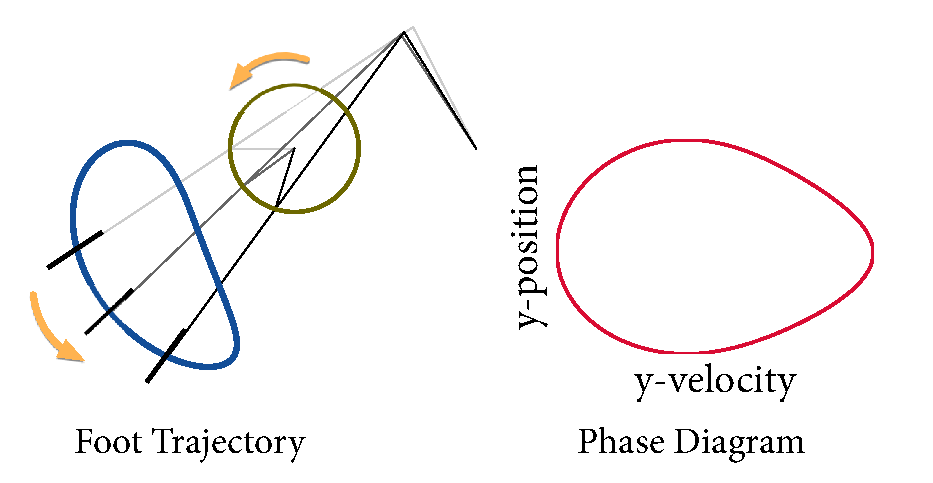
\includegraphics[width = \textwidth]{foot_traj_orig.eps}
    \caption{Real Foot locus and phase portrait.}% The circular path traced by end of the input link is traced in green.} 
    \label{fig:trajrob}
\end{subfigure}
\quad
\begin{subfigure}[t]{0.47\textwidth}
    \centering
    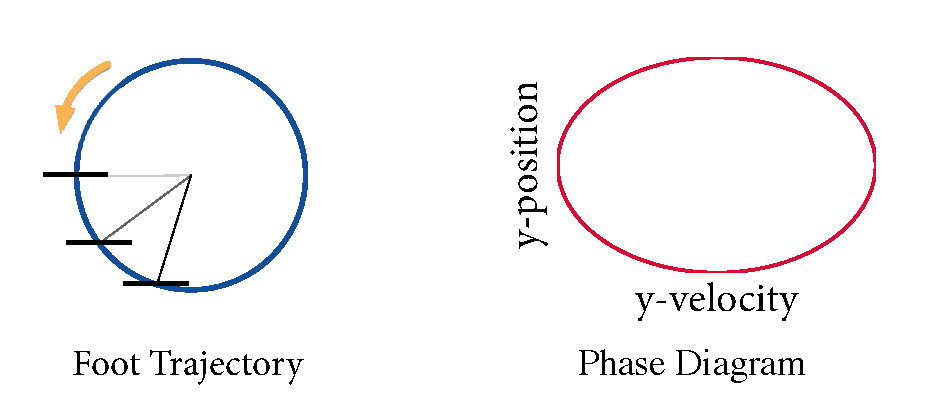
\includegraphics[width = \textwidth]{foot_traj_simple.eps}
    \caption{Simplified foot locus and phase portrait.} 
    \label{fig:trajsimp}
\end{subfigure}
\vspace{0.5EX}
\caption{Real and simplified leg trajectories (blue) and phase portraits (red).}
\label{fig:traj}
\end{figure}
\vspace{2EX}

\textcolor{prime}{\textsf{Leg Model}}
\begin{itemize}
    \item Only considers average vertical forces generated in one cycle of simplified trajectory
    \item Assumes velocity of leg $\gg$ of body oscillations
    \item Allows for different foot velocties during downwards and upwards phases of trajectory
    \item We integrate the following force equation~\cite{glasheen1996vertical} over simplified trajectory
        \begin{equation}
            F(t) = - C_D^* \left[\frac{1}{2} S \rho \dot{y}_f(t) |\dot{y}_f(t) | + S \rho g y_f(t) \right]
            \label{eq:force_t}
        \end{equation}
\hspace{1EM} \small{$C_D^*$ coefficient of friction, $S$ area of foot, $\rho$ density, $y_f$ position of foot, $g$ gravity}
\end{itemize}
\vspace{1EX}

\textcolor{prime}{\textsf{Robot Model}} \\
We linearize the result of integrating equation~\ref{eq:force_t} and write the height and roll dynamics in the form

\begin{equation}
    M \ddot{\vec{y}} = A \vec{y} + G + B \vec{\omega} 
    \label{eq:rob_dyn}
\end{equation}

\hspace{1EM} $\vec{y} = [y, \theta]^T = $\  height and roll \\

\hspace{1EM} $\vec{\omega} = [\omega^-_l, \omega^+_l, \omega^-_r, \omega^+_r]^T = $\ downwards and upwards leg frequencies for left \\ \hspace{1EM} and right sides of robot

            \end{block}
        \end{column}
        \begin{column}{.3\linewidth}
            \begin{block}{Controller Design}
                \textcolor{prime}{\textsf{Central Pattern Generator (CPG)}} \\
\begin{figure}[h]
	\centering
    \includegraphics[height=2.9in]{cpg-crop.pdf}
    \caption{The CPG helps maintain a trot gait. Blue circles represent leg osccilators, black arrows represent phase couplings, and red arrows represent external forcing terms.}
    \label{fig:CPG_Network}
\end{figure}
\vspace{-0.25in}

\vspace{1EX}
\textcolor{prime}{\textsf{Inverse Dynamics}} \\
\begin{itemize}
\item We use an inverse dynamics approach to reject disturbances
\item Formulation: Obtain desired acceleration via task-space PID. Plug into equation~\ref{eq:rob_dyn} and solve for control input $\vec{\omega}$

    \begin{equation*}
        \vec{\omega} = B^{\dagger} \left[M \mathrm{PID}(\vec{y}_d - \vec{y})- A \vec{y} - G \right] + (\mathbbm{1} - B^{\dagger} B) \vec{\omega}_0 \label{eq:control}
    \end{equation*}

\item We use a heuristic to set $\vec{\omega}_0$ at each time step so that the nullspace is used to find control inputs that help the system converge to trot gait
\begin{equation}
    \vec{\omega}_0^{t+1} = \underbrace{\frac{1}{2}\begin{bmatrix}
        {\omega_l^-}^t + {\omega_l^+}^t \\
        {\omega_l^-}^t + {\omega_l^+}^t \\
        {\omega_r^-}^t + {\omega_r^+}^t \\
        {\omega_r^-}^t + {\omega_r^+}^t \\
    \end{bmatrix}}_{\text{term 1}} + 
    \underbrace{\vphantom{\frac{1}{2}\begin{bmatrix}
        {\omega_l^-}^t + {\omega_l^+}^t \\
        {\omega_l^-}^t + {\omega_l^+}^t \\
        {\omega_r^-}^t + {\omega_r^+}^t \\
        {\omega_r^-}^t + {\omega_r^+}^t \\
    \end{bmatrix}}
    k \begin{bmatrix}
        \sin \left( \phi_r^t - \phi_l^t - \pi \right) \\
        \sin \left( \phi_r^t - \phi_l^t - \pi \right) \\
        \sin \left( \phi_l^t - \phi_r^t + \pi \right) \\
        \sin \left( \phi_l^t - \phi_r^t + \pi \right) \\
    \end{bmatrix}}_{\text{term 2}}
    \label{eq:hu}
\end{equation}

\item Term 1: leg speeds at the next timestep are close to those at the last time step
\item Term 2: leg speeds that help bring the robot back to a trot gait
\end{itemize}

            \end{block}
            \begin{block}{Simulation Results}
                In order to control the roll and pitch angles of the robot, we must be able to control the height of each corner of the robot. We have achieved preliminary results controlling the height of a one legged hopping robot using the nonlinear control outlined in the previous section. We have found that adding PID to this control scheme in an outer loop can reduce setting time, oscillations about the desired height, and steady state error.

            \end{block}
        \end{column}
        \begin{column}{.3\linewidth}
            \begin{block}{Conclusion}
                \textcolor{prime}{\textsf{Findings}} \\
\begin{itemize}
\item When we only use the first term of the heuristic, (equation~\ref{fig:woheu}),  the system can leave a trot gait and quickly becomes unstable at higher amplitude disturbances.

\item When we use both terms of the heuristic the system can reject higher amplitude disturbances because it is able to maintain a trot gait. 

\item System can still be forced to leave a trot gait if disturbance is large enough
\end{itemize}

\vspace{2EX}
\textcolor{prime}{\textsf{Future Work}} \\
\begin{itemize}
	\item Test the controller on a real robot to verify its rohbustness given:
	\begin{itemize}
		\item motor dynamics
		\item waves produced by feet
		\item sensor noise
	\end{itemize}
	\item Rotating boom setup will allow the robot to run in a circle in a small pool. 
\end{itemize}

\vspace{2EX}
\begin{figure}[htb]
    \centering
	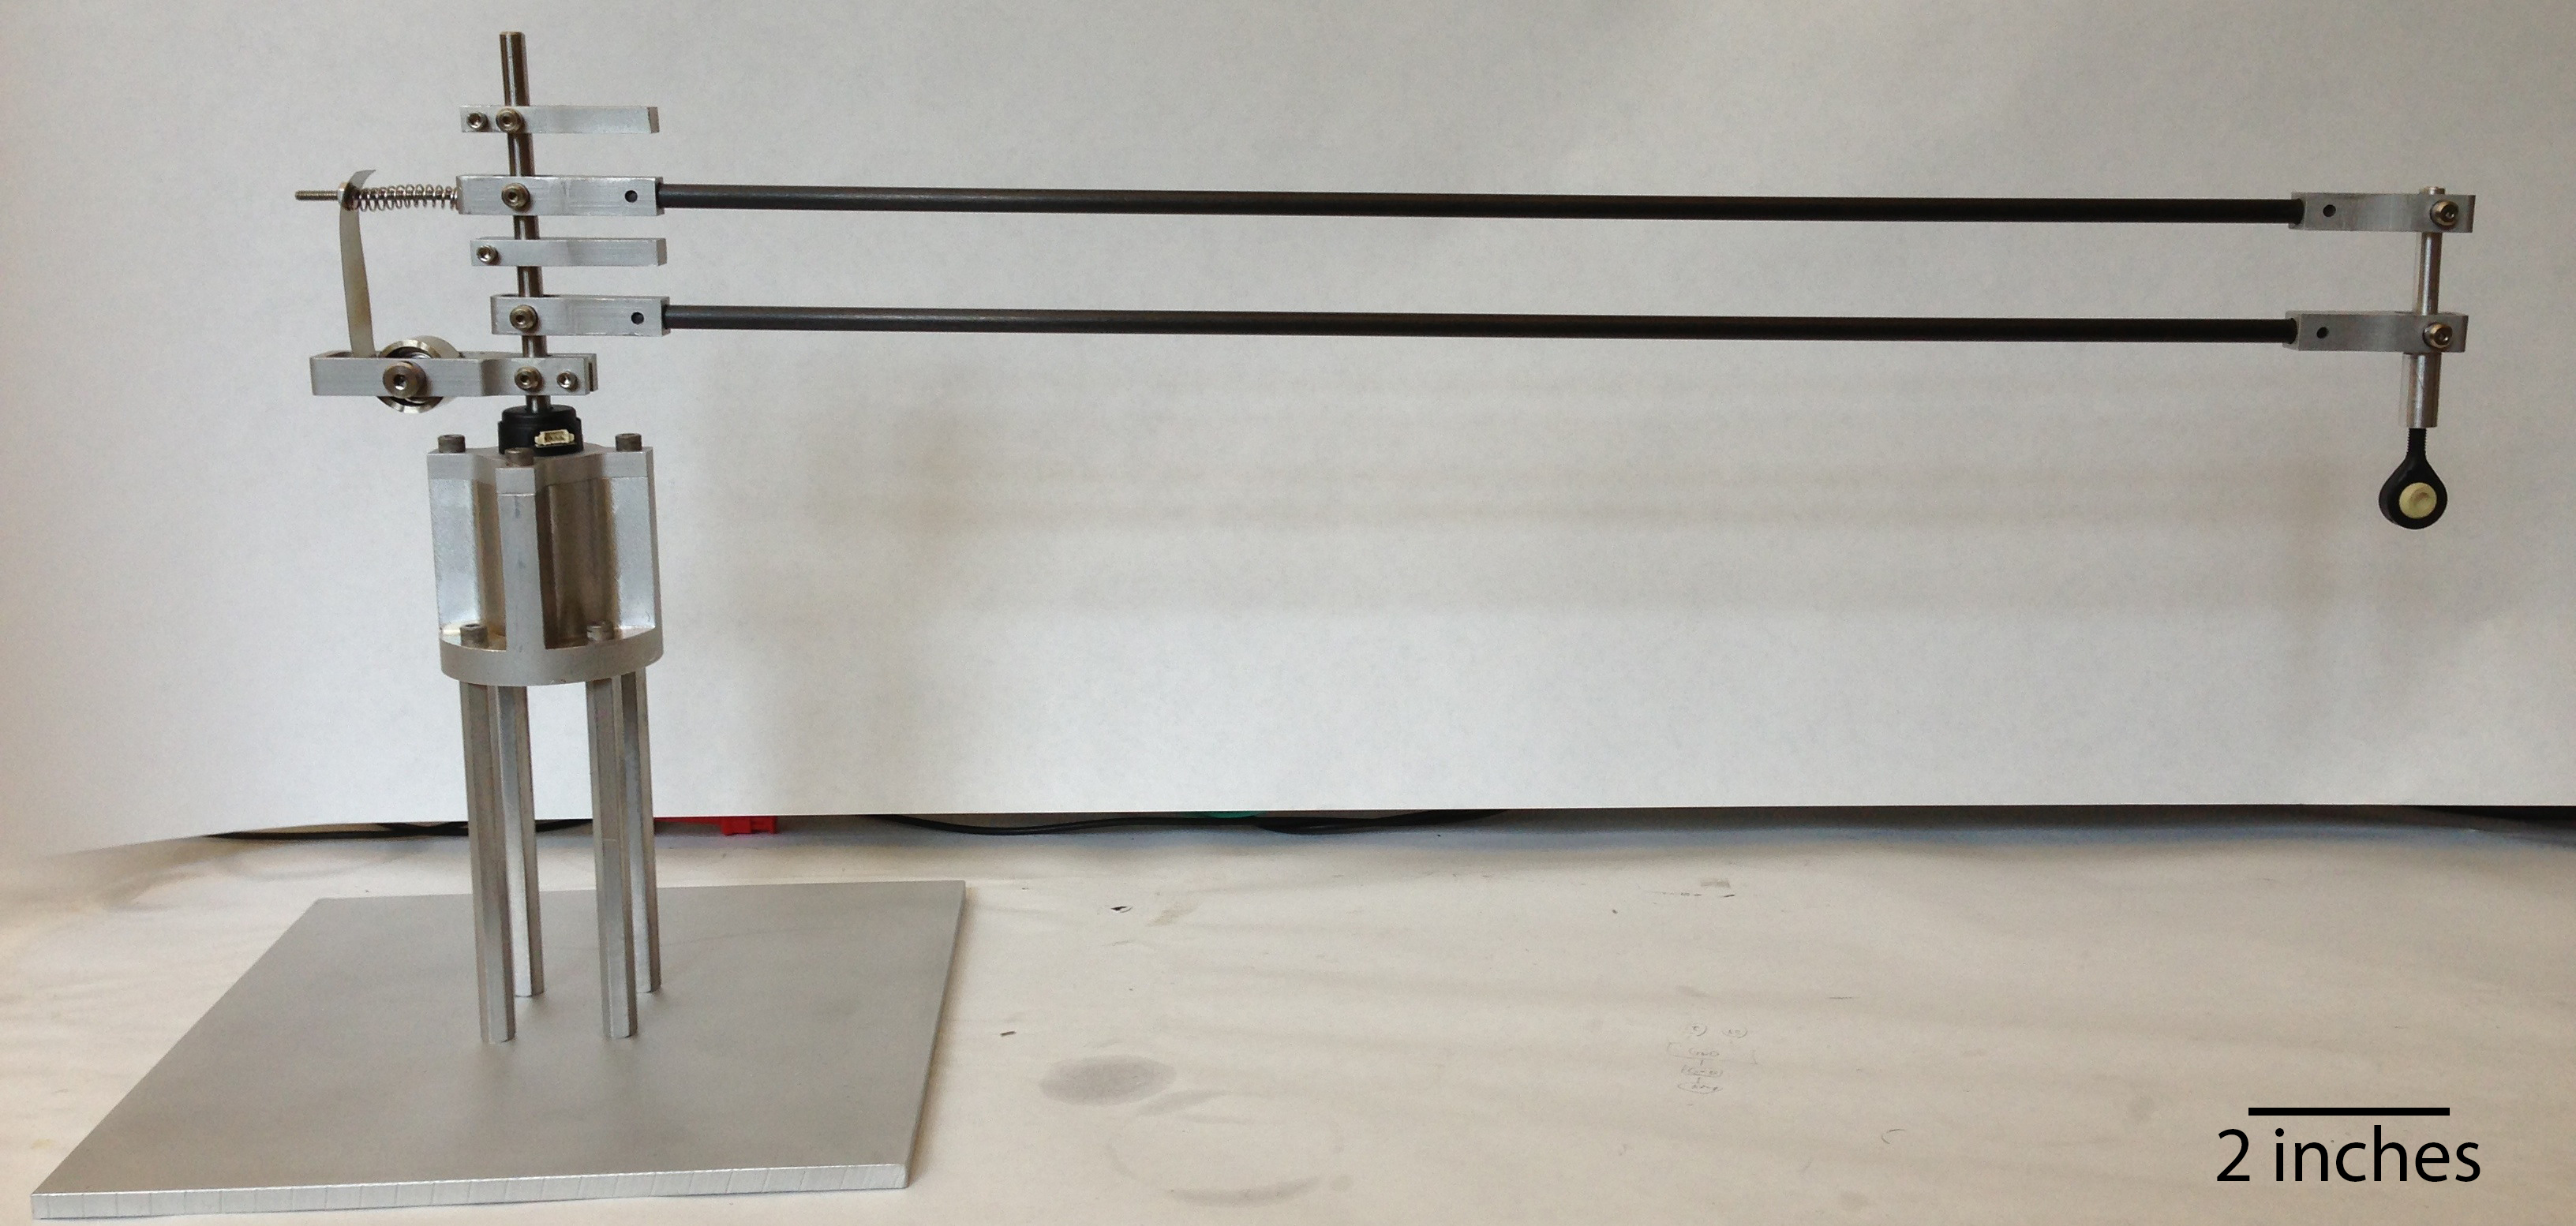
\includegraphics[height = 6in]{boom.jpg}
    \caption{Robot with testing boom (placeholder)}
\end{figure}
\vspace{-1in}

            \end{block}
            \vspace{0.5in}

            \begin{block}{Acknowledgement}
                \small
                This material is based upon work supported by the National Science Foundation Graduate Research Fellowship under Grant No. (0946825).

            \end{block}

            \vspace{0.5in}
            \begin{block}{References}
                \small
                \setbeamertemplate{bibliography item}[text] 
                \bibliographystyle{IEEEtran}
                \bibliography{ref}
            \end{block}
        \end{column}
    \end{columns}
\end{frame}
\end{document}
